\chapter{Ergebnisse und Bewertung}\label{chap:ergebnisse_und_bewertung}

In diesem Kapitel werden die Ergebnisse der in \cref{chap:konzeption} vorgestellten Verfahren präsentiert. Zunächst wird die SDE-basierte Aktienauswahl durchgeführt, um aus dem S\&P500-Universum zehn Aktien für die weitere Analyse zu selektieren. Anschließend werden die Vorhersagemodelle auf diesen Aktien evaluiert.

\section{SDE Aktienauswahl}\label{sec:sde}

Das in \cref{subsec:aktienauswahl} beschriebene Verfahren zur Aktienauswahl wurde auf dem S\&P500-Universum (Stand Januar 2020) angewendet. Es wurden Kursdaten, sowie die Preisdaten der sechs makroökonomischen Faktoren aus \cref{tab:makrofaktoren} für den Trainingszeitraum (01.2020--12.2023) geladen.

\subsection{Dominante Faktorpaare}

Im ersten Schritt wurde für jede Aktie mittels OLS-Regression das dominante Faktorpaar bestimmt. Die Summe der Betragskoeffizienten $|\beta_{i,j}| + |\beta_{i,k}|$ gibt an, wie stark die diskretisierten Kursbewegungen der Aktie mit den beiden Faktoren korrelieren. \cref{tab:beta_beispiele} zeigt einen Ausschnitt der Aktien mit den höchsten Beta-Summen.

\begin{table}[h!]
    \centering
    \begin{tabular}{l c c c}
        Ticker & Faktor 1 & Faktor 2 & $\sum|\beta|$ \\
        \hline
        MSFT   & Staatsanleihe & S\&P500  & 0,661 \\
        TEL    & Gold     & S\&P500  & 0,656 \\
        MCO    & Staatsanleihe & S\&P500  & 0,647 \\
        ACN    & Staatsanleihe & S\&P500  & 0,641 \\
        TXN    & Öl       & S\&P500  & 0,638 \\
        AAPL   & Staatsanleihe & S\&P500  & 0,628 \\
        AMP    & Staatsanleihe & S\&P500  & 0,628 \\
        APA    & Öl       & S\&P500  & 0,626 \\
        \hline
    \end{tabular}
    \caption{Aktien mit höchsten Beta-Summen (Ausschnitt)}\label{tab:beta_beispiele}
\end{table}

Die Verteilung der dominanten Faktorpaare über alle Aktien zeigt, dass der S\&P500-Index in fast allen Kombinationen vertreten ist (\cref{tab:faktorpaar_verteilung}). Dies entspricht der Erwartung, dass Aktien innerhalb des Index stark mit dem Gesamtmarkt korrelieren.

\begin{table}[h!]
    \centering
    \begin{tabular}{l c c}
        Faktorpaar & Anzahl Aktien & Anteil \\
        \hline
        Staatsanleihe, S\&P500   & 179 & 39,8\,\% \\
        Dollar, S\&P500     & 139 & 30,9\,\% \\
        Öl, S\&P500         & 86  & 19,1\,\% \\
        Gold, S\&P500       & 30  & 6,7\,\%  \\
        Inflation, S\&P500  & 14  & 3,1\,\%  \\
        Gold, Öl            & 2   & 0,4\,\%  \\
        \hline
    \end{tabular}
    \caption{Verteilung der dominanten Faktorpaare}\label{tab:faktorpaar_verteilung}
\end{table}

\subsection{Euler-Maruyama Simulation}

Nach der Gruppierung wurden 100 Monte-Carlo-Simulationen durchgeführt. In jeder Simulation wurden Gruppen aus je vier Aktien mit gemeinsamem Faktorpaar gebildet und deren Kursverläufe über 378 Handelstage, also dem gesamten Testzeitraum simuliert.

\cref{fig:sde_simulation} zeigt exemplarisch eine solche Simulation für eine Gruppe mit den dominanten Faktoren Gold und S\&P500. Die Kurse sind auf einen Startwert von 100 normalisiert, um die relativen Entwicklungen vergleichbar zu machen. Die durchgezogenen Linien zeigen die simulierten Aktienkurse, die gestrichelten Linien die Faktorverläufe.

\begin{figure}[htbp]
    \centering
    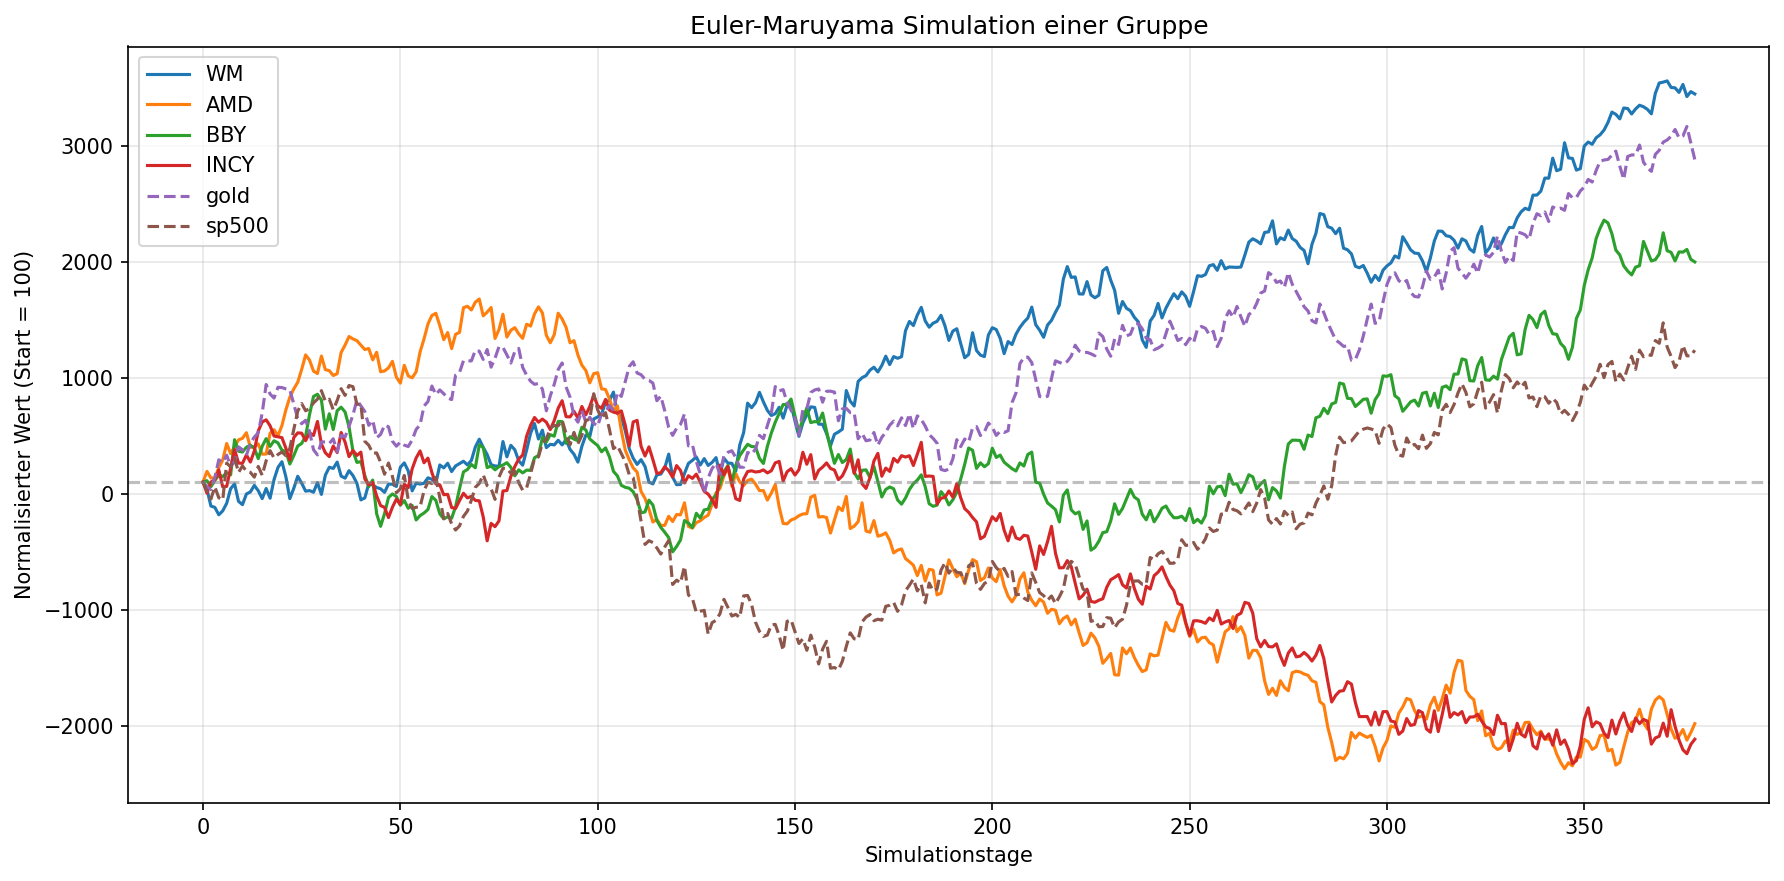
\includegraphics[width=\textwidth]{Bilder/sde_example_simulation.png}
    \caption{Beispielhafte Euler-Maruyama Simulation einer Gruppe}\label{fig:sde_simulation}
\end{figure}

\subsection{Vorhergesagte ROI und Ranking}

Für jede Aktie wurde über alle Simulationen der durchschnittliche \ac{ROI} berechnet. \cref{tab:top_roi} zeigt die zehn Aktien mit den höchsten durchschnittlichen simulierten ROIs.

\begin{table}[h!]
    \centering
    \begin{tabular}{c l c c}
        Rang & Ticker & Faktorpaar & Avg. sim. ROI \\
        \hline
        1  & RSG  & Inflation, S\&P500 & 24,50\,\% \\
        2  & AJG  & Dollar, S\&P500   & 25,39\,\% \\
        3  & CTAS & Dollar, S\&P500   & 24,48\,\% \\
        4  & TT   & Dollar, S\&P500   & 23,39\,\% \\
        5  & GOOG & Inflation, S\&P500 & 23,21\,\% \\
        6  & ABBV & Staatsanleihe, S\&P500 & 22,92\,\% \\
        7  & PEP  & Staatsanleihe, S\&P500 & 22,92\,\% \\
        8  & GWW  & Öl, S\&P500       & 22,74\,\% \\
        9  & CARR & Öl, Gold          & 22,68\,\% \\
        10 & ORLY & Gold, S\&P500     & 21,65\,\% \\
        \hline
    \end{tabular}
    \caption{Top 10 Aktien nach durchschnittlichem simuliertem ROI}\label{tab:top_roi}
\end{table}

Da es um einen qualitativen Vergleich der Aktienverläufe geht, ergibt sich die finale Auswahl aus der durchschnittlichen Platzierung über alle Simulationsrunden. Eine Aktie, die häufig als Gewinner ihrer Gruppe hervorgeht, erhält eine bessere Durchschnittsplatzierung. Dies führt zu dem in \cref{tab:selected_stocks} dargestellten Ergebnis.

\subsection{Ausgewählte Aktien}

Die durch das SDE-Verfahren ausgewählten zehn Aktien werden in \cref{tab:selected_stocks} mit vollständigem Namen und Branche dargestellt. Diese Aktien bilden die Grundlage für die Evaluation der Vorhersagemodelle im Testzeitraum.

\begin{table}[h!]
    \centering
    \begin{tabular}{c l l l}
        Rang & Ticker & Unternehmen & Branche \\
        \hline
        1  & CARR & Carrier Global Corp.      & Industrie \\
        2  & OTIS & Otis Worldwide Corp.      & Industrie \\
        3  & RSG  & Republic Services Inc.    & Abfallentsorgung \\
        4  & CTAS & Cintas Corp.              & Dienstleistungen \\
        5  & AJG  & Arthur J. Gallagher \& Co. & Versicherungen \\
        6  & PEP  & PepsiCo Inc.              & Konsumgüter \\
        7  & TT   & Trane Technologies        & Industrie \\
        8  & GWW  & W.W. Grainger Inc.        & Handel \\
        9  & RMD  & ResMed Inc.               & Medizintechnik \\
        10 & BLK  & BlackRock Inc.            & Finanzdienstleistungen \\
        \hline
    \end{tabular}
    \caption{Die zehn ausgewählten Aktien}\label{tab:selected_stocks}
\end{table}

Ausführlichere Ergebnisse der Aktienauswahl, einschließlich der dominanten Faktorpaare, Beta-Summen und durchschnittlichen ROIs für die analysierten Aktien, sind in \cref{app:selection_results} zu finden. TODO:Anhang ist nicht vollständig. Entweder sagen dass da auch nicht alle sind, oder alle reinmachen.

\section{LinearSeparation}\label{sec:linearseparation}

% TODO: Ergebnisse des LinearSeparation-Modells auf den ausgewählten Aktien


In diesem Abschnitt werden die Ergebnisse des in \cref{subsec:linearesModell} vorgestellten LinearSeparation-Modells präsentiert. Das Modell wurde auf den zehn durch das SDE-Verfahren ausgewählten Aktien im Testzeitraum (07.2024--12.2025) evaluiert.

Wie in \cref{subsec:signal} beschrieben, wird der Schwellenwert $\varepsilon$ für das Handelssignal aus dem \ac{MAE} auf den Validierungsdaten bestimmt. \cref{tab:ls_epsilon} zeigt die ermittelten Schwellenwerte für jede Aktie. Die Werte für das Modell variieren zwischen 0,44\% und 2,76\%.

\begin{table}[h!]
    \centering
    \begin{tabular}{l c}
        \toprule
        Ticker & $\varepsilon$ \\
        \midrule
        CARR & 1,58\% \\
        OTIS & 1,37\% \\
        RSG  & 2,28\% \\
        CTAS & 1,34\% \\
        AJG  & 1,38\% \\
        PEP  & 2,32\% \\
        TT   & 2,45\% \\
        GWW  & 0,44\% \\
        RMD  & 2,76\% \\
        BLK  & 1,46\% \\
        \midrule
        \O   & 1,74\% \\
        \bottomrule
    \end{tabular}
    \caption{Schwellenwerte $\varepsilon$ für das Handelssignal pro Aktie}\label{tab:ls_epsilon}
\end{table}

Aktien mit höherer Volatilität wie RMD weisen einen größeren Schwellenwert auf, da das Modell hier größere Prognosefehler produziert. Niedrigere Schwellenwerte bei Aktien wie GWW führen zu häufigeren Handelssignalen.


Die Vorhersagequalität des LinearSeparation-Modells wird anhand der in \cref{subsec:fehlermasse} definierten Fehlermaße bewertet. \cref{tab:ls_fehler} fasst die Ergebnisse zusammen.

\begin{table}[h!]
    \centering
    \begin{tabular}{l S[table-format=1.2] S[table-format=-1.2] S[table-format=1.2]}
        \toprule
        Ticker & {MAPE (\%)} & {OOS-$R^2$} & {DA} \\
        \midrule
        CARR & 1,53 & -0,08 & 0,47 \\
        OTIS & 1,02 & -0,14 & 0,48 \\
        RSG  & 0,83 & -0,06 & 0,56 \\
        CTAS & 1,01 & -0,07 & 0,55 \\
        AJG  & 1,13 & -0,15 & 0,53 \\
        PEP  & 0,97 & -0,07 & 0,48 \\
        TT   & 1,26 & -0,10 & 0,50 \\
        GWW  & 1,09 & -0,10 & 0,48 \\
        RMD  & 1,30 & -0,13 & 0,53 \\
        BLK  & 1,15 & -0,09 & 0,55 \\
        \midrule
        \O   & 1,13 & -0,10 & 0,51 \\
        \bottomrule
    \end{tabular}
    \caption{Fehlermaße des LinearSeparation-Modells im Testzeitraum}\label{tab:ls_fehler}
\end{table}

Der durchschnittliche MAPE von 1,13\% zeigt, dass die Vorhersagen im Mittel um etwa 1\% vom tatsächlichen Kurs abweichen. Die negativen OOS-$R^2$-Werte von durchschnittlich $-0,10$ deuten darauf hin, dass das Modell den Random-Walk-Benchmark nicht übertrifft. Es lässt sich beobachten dass die Vorhersagen häufig sehr nah an den Kursen vom Vortag liegen, was bedeutet dass das Modell zu stark interpoliert.

Die Directional Accuracy liegt mit durchschnittlich 51,3\% knapp über dem Zufallsniveau von 50\%. Einzelne Aktien wie RSG (56,1\%), CTAS (55,1\%) und BLK (54,8\%) zeigen eine leicht überdurchschnittliche Trefferquote bei der Richtungsvorhersage.

Die finanzwirtschaftliche Bewertung erfolgt anhand der in \cref{subsec:finanzkennzahlen} definierten Kennzahlen. \cref{tab:ls_trading} zeigt die Ergebnisse der simulierten Handelsstrategie mit einem Startkapital von 100.000 US\$.

\begin{table}[h!]
    \centering
    \begin{tabular}{l S[table-format=-2.2] S[table-format=2.2] S[table-format=-2.2] S[table-format=-2.2] S[table-format=2.2]}
        \toprule
        Ticker & {Return (\%)} & {B\&H (\%)} & {Excess (\%)} & {Sharpe} & {MDD (\%)} \\
        \midrule
        CARR & -7,00 & -12,29 & 5,29 & -0,36 & 26,46 \\
        OTIS & -21,02 & -4,88 & -16,14 & -27,93 & 24,44 \\
        RSG  & 19,93 & 13,11 & 6,82 & 1,08 & 8,55 \\
        CTAS & -3,46 & 11,02 & -14,48 & -0,76 & 23,58 \\
        AJG  & 19,00 & 2,30 & 16,70 & 2,49 & 9,95 \\
        PEP  & -13,00 & -6,47 & -6,52 & -5,06 & 18,21 \\
        TT   & 4,49 & 23,33 & -18,83 & 0,07 & 18,33 \\
        GWW  & 0,50 & 15,40 & -14,90 & -0,08 & 25,05 \\
        RMD  & 8,87 & 31,79 & -22,92 & 0,52 & 9,42 \\
        BLK  & 32,28 & 42,86 & -10,58 & 1,70 & 11,79 \\
        \midrule
        \O   & 4,06 & 11,62 & -7,56 & -2,83 & 17,58 \\
        \bottomrule
    \end{tabular}
    \caption{Trading-Performance des LinearSeparation-Modells}\label{tab:ls_trading}
\end{table}

Die durchschnittliche Gesamtrendite beträgt 4,06\%, was unter der Buy-and-Hold-Rendite von 11,62\% liegt. Die Excess-Rendite von durchschnittlich $-7,56\%$ zeigt, dass die aktive Strategie im Mittel schlechter abschneidet als ein passives Investment.

Einzelne Aktien zeigen positive Excess-Renditen:
\begin{itemize}
    \item \textbf{AJG:} +16,70\% Excess-Rendite bei positivem Sharpe Ratio von 2,49
    \item \textbf{RSG:} +6,82\% Excess-Rendite bei Sharpe Ratio von 1,08
    \item \textbf{CARR:} +5,29\% Excess-Rendite trotz negativer Gesamtrendite
\end{itemize}

Der durchschnittliche Maximum Drawdown von 17,58\% zeigt das Risiko der Strategie. Die niedrigsten Drawdowns treten bei RSG (8,55\%) und RMD (9,42\%) auf, während CARR (26,46\%) und GWW (25,05\%) die höchsten Verlustphasen aufweisen.

\cref{fig:walkforward_rmd} zeigt exemplarisch den Walk-Forward-Backtest für die Aktie RMD. Im oberen Teil ist der Portfoliowert über den Testzeitraum dargestellt, im unteren Teil der Aktienkurs zusammen mit den Vorhersagen und Handelssignalen. Die Visualisierung zeigt wiederholt, wie nah die Vorhersagen an den jeweiligen Kursen des Vortages orientiert sind.

\begin{figure}[htbp]
    \centering
    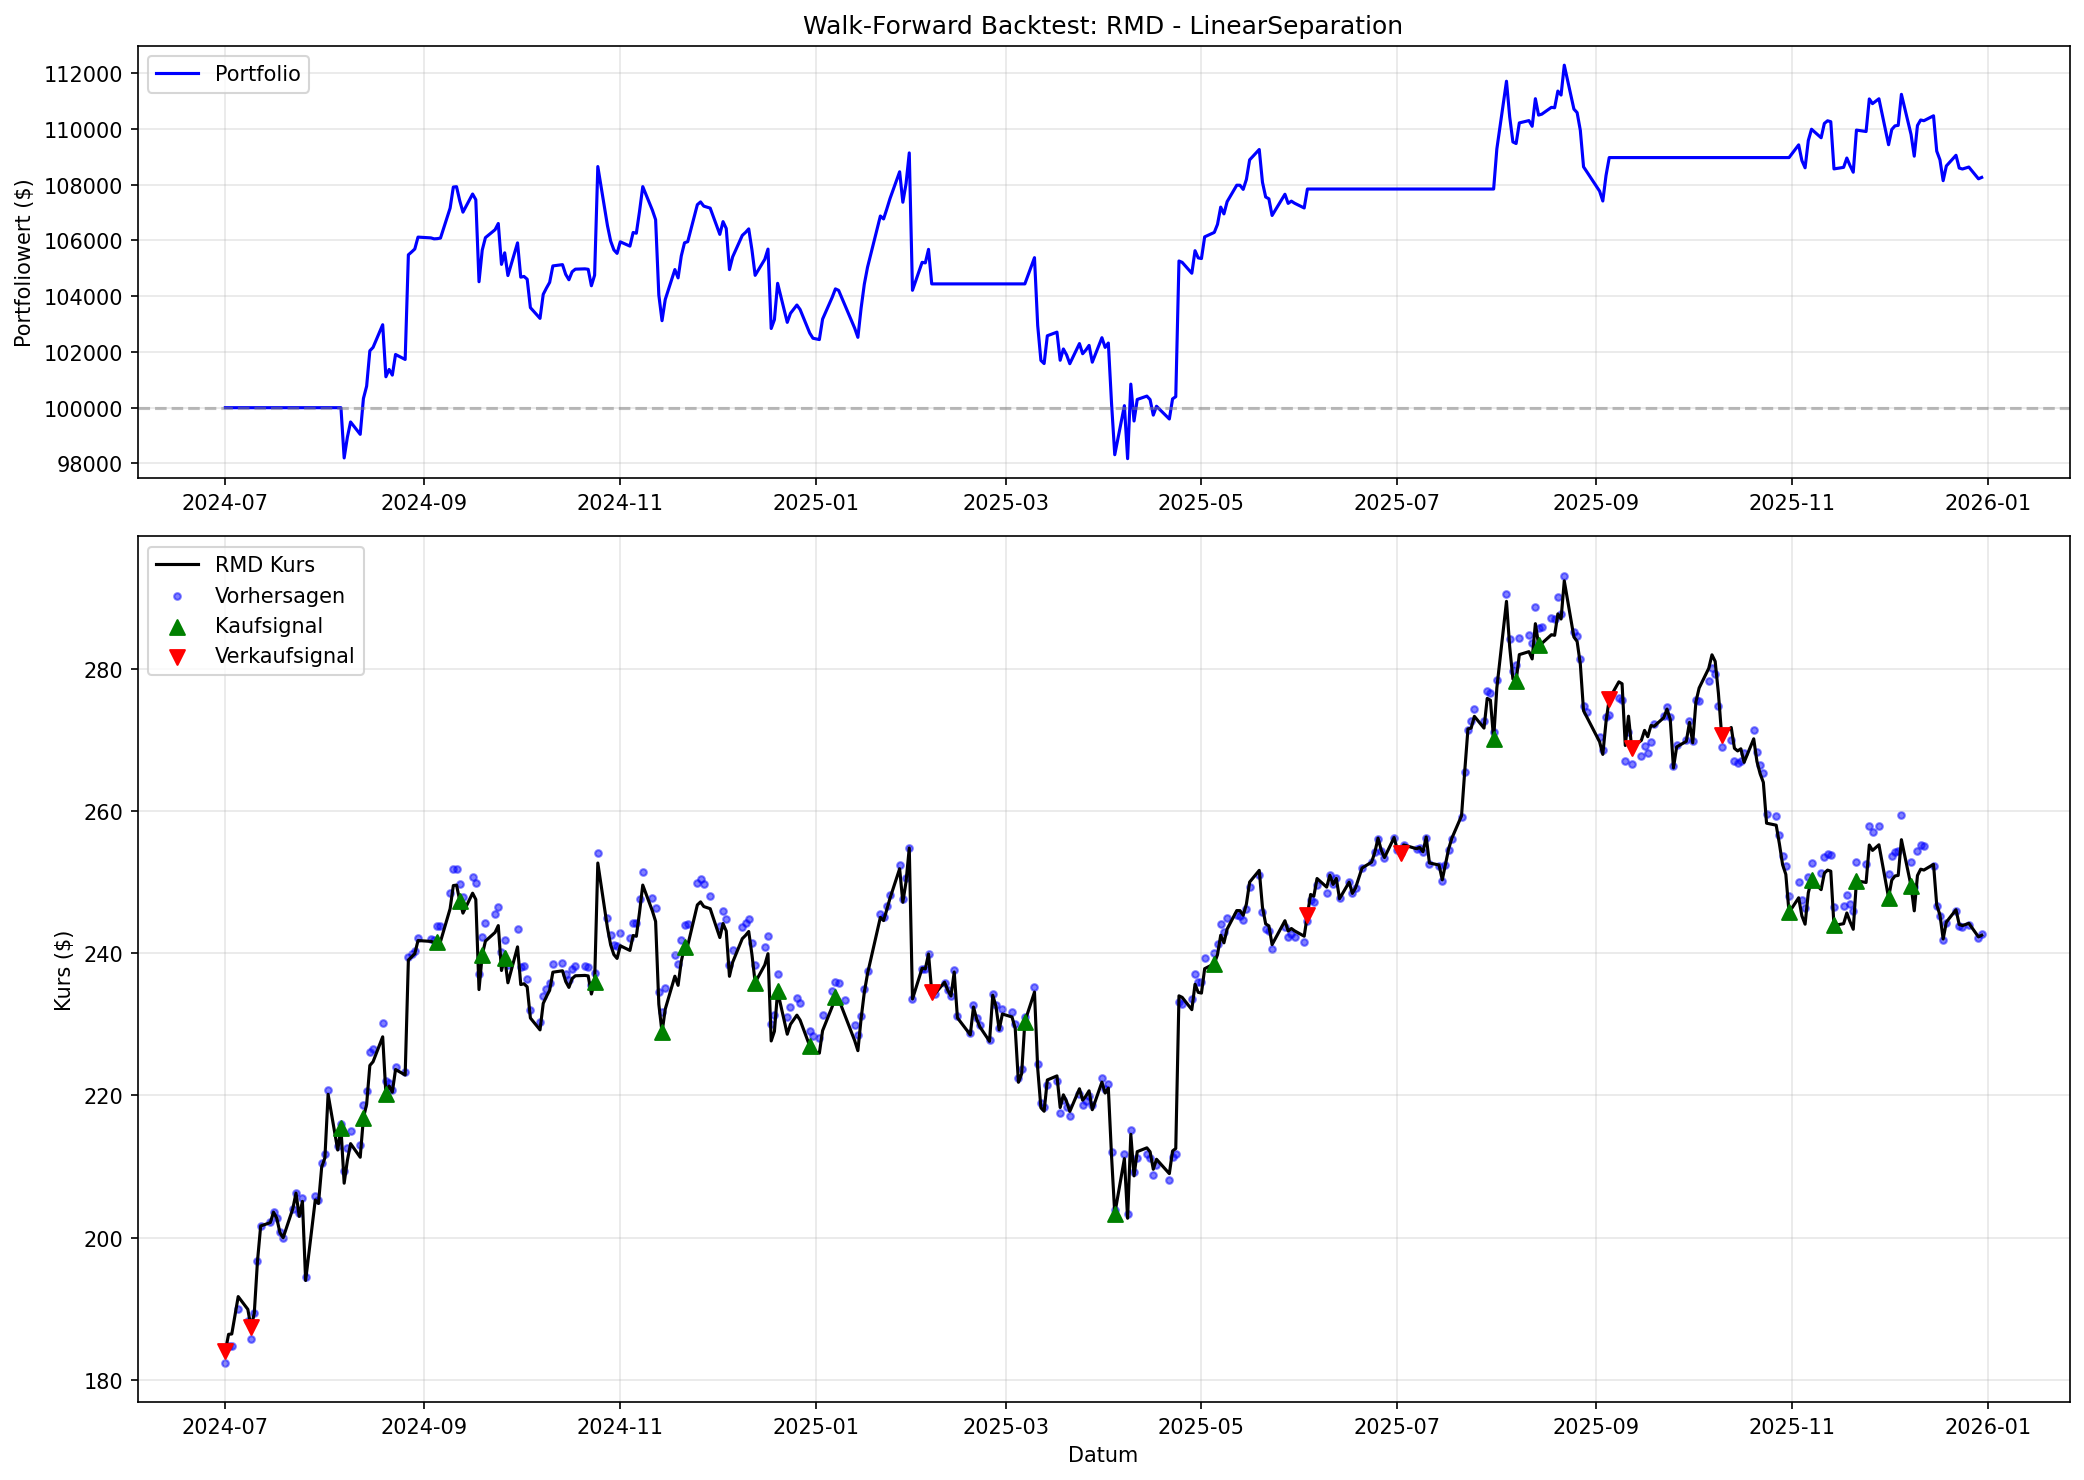
\includegraphics[width=\textwidth]{Bilder/walkforward_RMD_LinearSeparation.png}
    \caption{Walk-Forward-Backtest für RMD mit LinearSeparation-Modell. Oben: Portfoliowert. Unten: Aktienkurs (schwarz), Vorhersagen (blau), Kaufsignale (grün), Verkaufssignale (rot).}\label{fig:walkforward_rmd}
\end{figure}




\section{Preprocessed SVR}\label{sec:svr}

% TODO: Ergebnisse des SVR-Modells auf den ausgewählten Aktien

\section{TimesFM}\label{sec:stocktimesfm}

% TODO: Ergebnisse des TimesFM-Modells auf den ausgewählten Aktien
